\chapter{Quiz}
\newpage
\section*{Quiz 1}
\begin{exercise}{เขียนแบบจำลองและแก้ปัญหาด้วยการวาดรูป}{quiz1}
    บริษัทผลิตอัญมณีแห่งหนึ่งผลิตแหวนและต่างหูจากแร่เงินและแร่ทองคำ โดยที่
    \begin{itemize}
        \item ในการผลิตแหวน จะต้องใช้แร่งทองคำ 3 หน่วย และแร่เงิน 3 หน่วย และจะขายได้กำไร 2 พันบาท
        \item ในการผลิตต่างหู จะต้องใช้แร่งทองคำ 1 หน่วย และแร่เงิน 5 หน่วย และจะขายได้กำไร 1 พันบาท
    \end{itemize}
    ในรอบการผลิตปัจจุบัน บริษัทนี้ได้รับแร่ทองคำมา 18 หน่วย และแร่เงินมา 30 หน่วย โดยที่บริษัทอยากผลิตแหวนและต่างหูให้ได้กำไรมากที่สุด
\end{exercise}

\begin{enumerate}[label=\textbf{ขั้นที่ \arabic*:}, align=left, labelwidth=5em, labelsep=1em, leftmargin=*, itemsep=16pt, topsep=0pt, parsep=0pt, partopsep=0pt]
    \item กำหนดตัวแปร โดยกำหนดให้ $x = \text{จำนวนแหวนที่จะผลิต}$ และ $y = \text{จำนวนต่างหูที่จะผลิต}$
    \item เขียนฟังก์ชันจุดประสงค์ โดยสิ่งที่เป็นเป้าหมายของโจทย์ธุรกิจนี้คืออยาก \blank[1]{1cm} (max ตอบ 0 / min ตอบ 1) ค่ากำไรที่ได้จากการขาย โดยที่
\begin{equation}
    \text{กำไร} = \blank[2]{1.5cm}\ x + \blank[3]{1.5cm}\ y \tag{1}
\end{equation}
    \item เขียนอสมการเงื่อนไข โดยจากโจทย์จะได้ว่ามีเงื่อนไขอยู่ 2 เงื่อนไข คือเงื่อนไขการใช้แร่ทองคำ และเงื่อนไขการใช้แร่เงิน
        \begin{align}
            \text{แร่ทองคำ: }& &\blank[4]{1.5cm}\ x + \blank[5]{1.5cm}\  y &\leq \blank[6]{1.5cm} \tag{2} \\
            \text{แร่เงิน: }& &\blank[7]{1.5cm}\ x + \blank[8]{1.5cm}\  y &\leq \blank[9]{1.5cm}\tag{3} 
        \end{align}
    \item วาดรูปภาพเงื่อนไขจะได้ดังรูปด้านล่างสุด แต่เราจะแบ่งเป็นขั้นตอนการคิดดังนี้
        \begin{enumerate}[label=\textbf{ขั้นที่ 4.\arabic*:}, align=left, itemsep=16pt, topsep=0pt, parsep=0pt, partopsep=0pt]
            \item วาดเส้นเงื่อนไขการใช้แร่ทองคำ (สมการ [2]) โดยการหาจุดตัดแกนทั้ง 2:
                \begin{itemize}[itemsep=16pt]
                    \item หาระยะตัดแกน $x$ โดยการแทน $y = 0$ จะได้สมการ $\blank[4]{1.5cm}\ x = \blank[6]{1.5cm}$
                            ทำให้ได้ว่า $\displaystyle x = \frac{\ \blank[6]{1.5cm}\ }{\ \blank[4]{1.5cm}\ } = \blank[10]{1.5cm} $\\
                            จึงได้ว่าจุดตัดแกน $x$ คือจุด $\left(6,0\right)$
                    \item และในทำนองเดียวกัน จะได้ว่าจุดตัดแกน $y$ คือจุด $\left(0,18\right)$
                \end{itemize}
            \item ในทำนองเดียวกัน เมื่อพิจารณาเงื่อนไขการใช้แร่เงิน (สมการ [3]) \\
                    จะได้ว่าตัดแกน $x$ ที่จุด $\left(10,0\right)$ และตัดแกน $y$ ที่จุด $\left(0,6\right)$
            \item หาจุดตัดระหว่างสมการเส้นขอบของ [2] และสมการเส้นขอบของ [3] จะได้ว่าตัดกันที่จุด $(5,3)$ (+1 คะแนนพิเศษสำหรับคนที่สามารถแก้ระบบสมการเพื่อหาจุดตัดด้วยตัวเองได้: เขียนกระดาษแนบรูปหรือไฟล์ pdf มา)\label{bonus}
        \end{enumerate}
    \item แทนค่าจุดมุมลงในฟังก์ชันจุดประสงค์เพื่อหาค่าแล้วเปรียบเทียบกันว่าจุดใดให้ค่าจุดประสงค์ \blank[11]{1.5cm} (มากสุด ตอบ 0/ น้อยสุด ตอบ 1)\\
    \begin{minipage}{0.35\textwidth}
    \centering
    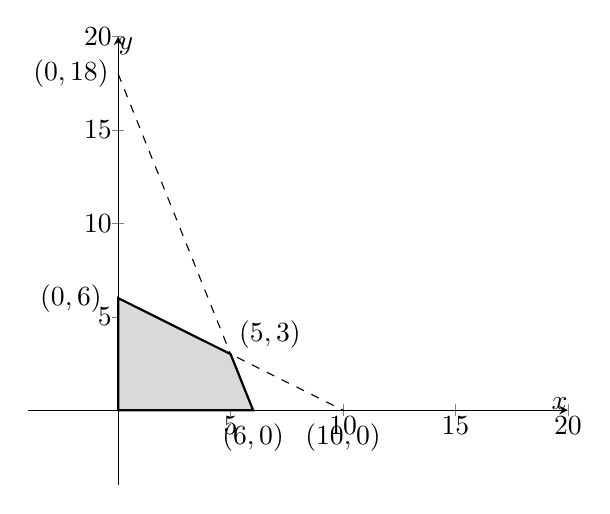
\begin{tikzpicture}[scale=1]
        \begin{axis}[
              axis lines=middle,
              xmin=-4, xmax=20,
              ymin=-4, ymax=20,
              xlabel={$x$}, ylabel={$y$},
            ]
            \addplot[black, dashed, domain=0:6] {18 - 3*x};
            \addplot[black, dashed, domain=0:10] {6 - 3/5*x};
            \addplot[black, thick, fill=gray!30] coordinates {(0,0) (0,6) (5,3) (6,0) (0,0)};
            \node at (axis cs:5,3) [xshift=0.5cm, yshift=0.25cm] {$(5,3)$};
            \node at (axis cs:6,0) [yshift=-0.35cm] {$(6,0)$};
            \node at (axis cs:0,18) [xshift=-0.6cm] {$(0,18)$};
            \node at (axis cs:0,6) [xshift=-0.6cm] {$(0,6)$};
            \node at (axis cs:10,0) [yshift=-0.35cm] {$(10,0)$};
        \end{axis}
    \end{tikzpicture}
\end{minipage}%
\hfill
\begin{minipage}{0.63\textwidth}
    \centering
    \begin{tabular}{c|c}
        $(x,y)$ & กำไร (จากสมการ [1]) \\
        \hline
        $(0,6)$ & \blank[14]{2cm} \\
        \hline
        $(6,0)$ & \blank[15]{2cm} \\
        \hline
        $(5,3)$ & \blank[16]{2cm} \\
        \hline
        $(\blank[12]{1cm},\blank[13]{1cm})$ & \blank[17]{2cm} \\
        \hline
    \end{tabular}
\end{minipage}

    \item สรุปคำตอบ จะได้ค่า \blank[11]{1.5cm} (มากสุด ตอบ 0/ น้อยสุด ตอบ 1) เท่ากับ \blank[18]{1cm} เกิดขึ้นที่จุด $(\blank[19]{1cm},\blank[20]{1cm})$
\end{enumerate}

\subsection*{โบนัสพิเศษ +1 คะแนน}
จงแสดงวิธีการระบบสมการในขั้นที่ \ref{bonus} ว่าได้จุดตัดเป็น $(5,3)$

\newpage
\section*{Quiz 2}
เราจะยังคงใช้โจทย์ปัญหาเดิมกับ quiz 1 อยู่
\begin{exercise}{simplex method}{quiz2}
    บริษัทผลิตอัญมณีแห่งหนึ่งผลิตแหวนและต่างหูจากแร่เงินและแร่ทองคำ โดยที่
    \begin{itemize}
        \item ในการผลิตแหวน จะต้องใช้แร่ทองคำ 3 หน่วย และแร่เงิน 3 หน่วย และจะขายได้กำไร 2 พันบาท
        \item ในการผลิตต่างหู จะต้องใช้แร่ทองคำ 1 หน่วย และแร่เงิน 5 หน่วย และจะขายได้กำไร 1 พันบาท
    \end{itemize}
    ในรอบการผลิตปัจจุบัน บริษัทนี้ได้รับแร่ทองคำมา 18 หน่วย และแร่เงินมา 30 หน่วย โดยที่บริษัทอยากผลิตแหวนและต่างหูให้ได้กำไรมากที่สุด
\end{exercise}

กำหนดให้ $x = \text{จำนวนแหวนที่จะผลิต}$ และ $y = \text{จำนวนต่างหูที่จะผลิต}$ และจาก quiz 1 เราได้โจทย์กำหนดการเชิงเส้นออกมาให้รูป

\begin{multicols}{2}
    \begin{align*}
    \max \quad & 2000x + 1000y\\
    \texttt{subject to} \quad
    & 3x + y \leq 18 \\
    & 3x + 5y \leq 30 \\
    & x \geq 0, \quad y \geq 0 
\end{align*}
และได้บริเวณการตัดสินใจเป็นตามรูปด้านขวา
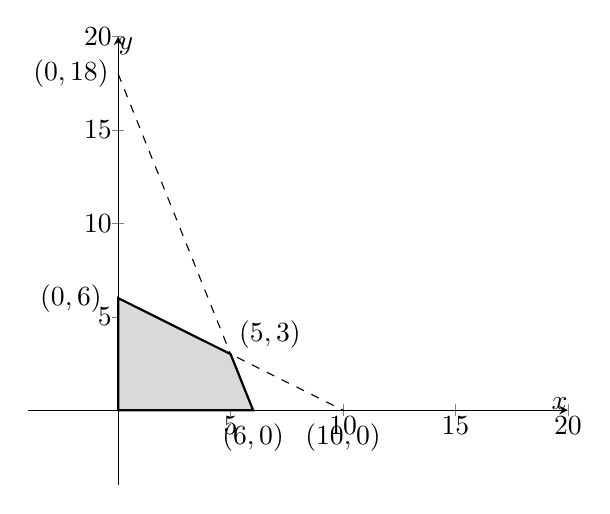
\begin{tikzpicture}[scale=1]
        \begin{axis}[
              axis lines=middle,
              xmin=-4, xmax=20,
              ymin=-4, ymax=20,
              xlabel={$x$}, ylabel={$y$},
            ]
            \addplot[black, dashed, domain=0:6] {18 - 3*x};
            \addplot[black, dashed, domain=0:10] {6 - 3/5*x};
            \addplot[black, thick, fill=gray!30] coordinates {(0,0) (0,6) (5,3) (6,0) (0,0)};
            \node at (axis cs:5,3) [xshift=0.5cm, yshift=0.25cm] {$(5,3)$};
            \node at (axis cs:6,0) [yshift=-0.35cm] {$(6,0)$};
            \node at (axis cs:0,18) [xshift=-0.6cm] {$(0,18)$};
            \node at (axis cs:0,6) [xshift=-0.6cm] {$(0,6)$};
            \node at (axis cs:10,0) [yshift=-0.35cm] {$(10,0)$};
        \end{axis}
    \end{tikzpicture}
\end{multicols}

\begin{multicols}{2}

    และจะแปลงเป็นรูปมาตรฐานได้ดังนี้
    \begin{align*}
        \max \quad & 2000x + 1000y + \blank[]{0.5cm}s_1+ \blank[]{0.5cm}s_2\\
        \texttt{s.t.} \quad
        & 3x + y + s_1 = 18 \\
        & 3x + 5y + s_2 = 30 \\
        & x \geq 0, \quad y \geq 0, \quad s_1 \geq 0, \quad s_2 \geq 0 
    \end{align*}
    และเมื่อนำมาเขียนตารางซิมเพลกซ์ตั้งต้นจะได้ดังนี้
    \begin{center}
        \begin{tabular}{|c|cccc|c|}
            \hline
            \textbf{Pivot} & $x$ & $y$ &  $s_1$ & $s_2$ &  \textbf{RHS} \\
            \hline
            $s_1$ & $3$ & $1$  & $1$ & $0$ & $\blank[]{0.5cm}$ \\
            $s_2$ & $\blank[]{0.5cm}$ & $\blank[]{0.5cm}$  & $\blank[]{0.5cm}$ & $\blank[]{0.5cm}$ & $\blank[]{0.5cm}$ \\
            \hline
            $z$   & $\blank[]{0.5cm}$ & $\blank[]{0.5cm}$  & $\blank[]{0.5cm}$ & $\blank[]{0.5cm}$ & $\blank[]{0.5cm}$ \\
            \hline
        \end{tabular}
    \end{center}
\end{multicols}

ต่อมาเป็นขั้นตอนการเปลี่ยนตัวแปรฐาน โดย
\begin{itemize}
    \item \textbf{ตัวแปรขาเข้า} โดยเลือกใช้ตัวแปรของคอลัมน์ที่มีค่าตัวเลขในแถว $z$ ติดลบมากที่สุด ซึ่งคือตัวแปร \blank[]{1cm}
    \item \textbf{ตัวแปรขาออก} โดยเลือกใช้ตัวแปรที่มีอัตราส่วนระหว่างค่าด้านขวามือ (RHS) กับสัมประสิทธิ์ของตัวแปรขาเข้าค่าบวกที่น้อยที่สุด
    \begin{center}
        \begin{tabular}{|c|cccc|c|c|}
            \hline
            \textbf{Pivot} & $x$ & $y$ &  $s_1$ & $s_2$ &  \textbf{RHS} & อัตราส่วน \\
            \hline
            $s_1$ & $3$ & $1$  & $1$ & $0$ & $\blank[]{0.5cm}$ & $\blank[]{0.5cm} {\Big /} \blank[]{0.5cm} = 6$ \\
            $s_2$ & $\blank[]{0.5cm}$ & $\blank[]{0.5cm}$  & $\blank[]{0.5cm}$ & $\blank[]{0.5cm}$ & $\blank[]{0.5cm}$ & $\blank[]{0.5cm} {\Big /} \blank[]{0.5cm} = 10$ \\
            \hline
            $z$   & $\blank[]{0.5cm}$ & $\blank[]{0.5cm}$  & $\blank[]{0.5cm}$ & $\blank[]{0.5cm}$ & $\blank[]{0.5cm}$ & \\
            \hline
        \end{tabular}
    \end{center}
    ดังนั้น จึงได้ว่าตัวแปรขาออกคือ \blank[]{1cm}
\end{itemize}
และเมื่อทำการดำเนินการตามแถวเพื่อเปลี่ยน pivot ตามขั้นตอนด้านล่างจะได้ตารางซิมเพลกซ์ใหม่ดังนี้
\begin{multicols}{2}
\noindent1. หารแถวของตัวแปรฐานใหม่ด้วยสัมประสิทธิ์ของตัวแปรฐานดังกล่าวในแถวนั้น\\
2. ดำเนินการตามแถวเพื่อให้สัมประสิทธิ์ของตัวแปรฐานในแถวอื่นเป็น 0\\
\begin{tabular}{|c|cccc|c|}
    \hline
    \textbf{Pivot} & $x$ & $y$ &  $s_1$ & $s_2$ &  \textbf{RHS}  \\
    \hline
    $x$ & $1$ & $1/3$  & $1/3$ & $0$ & $6$ \\
    $s_2$ & $0$ & $4$  & $-1$ & $1$ & $12$ \\
    \hline
    $z$   & $0$ & $-1000/3$  & $2000/3$ & $0$ & $12000$ \\
    \hline
\end{tabular}
\end{multicols}

\begin{multicols}{2}
    และถ้าทำซิมเพลกซ์ขั้นถัดไปจะได้ว่าต้องใช้ $y$ เป็นตัวแปรฐานขาเข้า และใช้ $s_2$ เป็นตัวแปรขาออก จะได้ตารางซิมเพลกซ์เป็น

    \begin{tabular}{|c|cccc|c|}
        \hline
        \textbf{Pivot} & $x$ & $y$ &  $s_1$ & $s_2$ &  \textbf{RHS}  \\
        \hline
        $x$ & $1$ & $0$  & $5/12$ & $-1/12$ & $5$ \\
        $y$ & $0$ & $1$  & $-1/4$ & $1/4$ & $3$ \\
        \hline
        $z$   & $0$ & $0$  & $1750/3$ & $250/3$ & $13000$ \\
        \hline
    \end{tabular}
\end{multicols}

ซึ่งไม่มีสมาชิกในแถว $z$ ติดลบแล้วจึงได้ว่ากระบวนการจบสิ้น ซึ่งจะได้ว่าผลเฉลยที่ทำให้ค่ามากสุดคือ $x = 5$ และ $y=3$ (ที่ได้จากคอลัมน์ RHS ในตารางสุดท้าย) และได้ $z = \blank[]{1.5cm}$ เป็นค่ามากสุด

\subsection*{โบนัสพิเศษ +1 คะแนน}
จงใช้ตาราง simplex สุดท้ายแปลงให้เป็นระบบสมการของตัวแปร $x, y, s_1, s_2$ และระบุเหตุผลว่าทำไม $x = 5$ และ $y=3$ โดยอาศัยตัวระบบสมการที่ได้ (คำใบ้: ตัวแปรที่ไม่ใช่ฐานคือตัวแปรที่โดนกำหนดให้ค่าเป็น 0 ดังนั้นต้องระบุให้ได้ก่อนว่าในตารางสุดท้ายใครถูกตั้งบทบาทให้เป็นตัวแปรฐาน)

\newpage
\begin{solution}
    กำหนดให้ $x = \text{จำนวนแหวนที่จะผลิต}$ และ $y = \text{จำนวนต่างหูที่จะผลิต}$ และจาก quiz 1 เราได้โจทย์กำหนดการเชิงเส้นออกมาให้รูป

\begin{multicols}{2}
    \begin{align*}
    \max \quad & 2000x + 1000y\\
    \texttt{subject to} \quad
    & 3x + y \leq 18 \\
    & 3x + 5y \leq 30 \\
    & x \geq 0, \quad y \geq 0 
\end{align*}
และได้บริเวณการตัดสินใจเป็นตามรูปด้านขวา
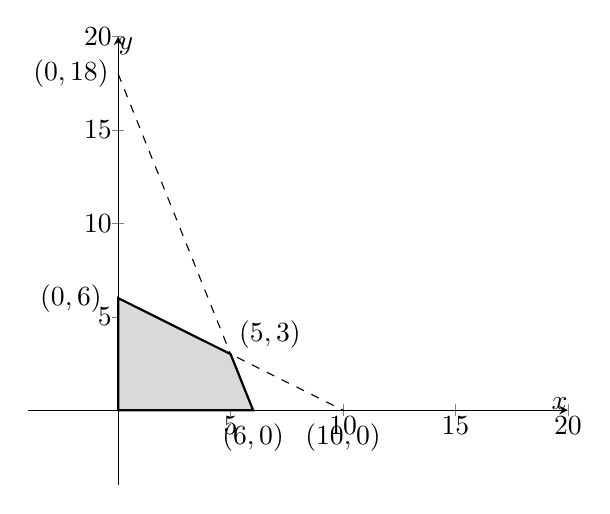
\begin{tikzpicture}[scale=1]
        \begin{axis}[
              axis lines=middle,
              xmin=-4, xmax=20,
              ymin=-4, ymax=20,
              xlabel={$x$}, ylabel={$y$},
            ]
            \addplot[black, dashed, domain=0:6] {18 - 3*x};
            \addplot[black, dashed, domain=0:10] {6 - 3/5*x};
            \addplot[black, thick, fill=gray!30] coordinates {(0,0) (0,6) (5,3) (6,0) (0,0)};
            \node at (axis cs:5,3) [xshift=0.5cm, yshift=0.25cm] {$(5,3)$};
            \node at (axis cs:6,0) [yshift=-0.35cm] {$(6,0)$};
            \node at (axis cs:0,18) [xshift=-0.6cm] {$(0,18)$};
            \node at (axis cs:0,6) [xshift=-0.6cm] {$(0,6)$};
            \node at (axis cs:10,0) [yshift=-0.35cm] {$(10,0)$};
        \end{axis}
    \end{tikzpicture}
\end{multicols}

\begin{multicols}{2}

    และจะแปลงเป็นรูปมาตรฐานได้ดังนี้
    \begin{align*}
        \max \quad & 2000x + 1000y + \blank[0]{0.5cm}s_1+ \blank[0]{0.5cm}s_2\\
        \texttt{s.t.} \quad
        & 3x + y + s_1 = 18 \\
        & 3x + 5y + s_2 = 30 \\
        & x \geq 0, \quad y \geq 0, \quad s_1 \geq 0, \quad s_2 \geq 0 
    \end{align*}
    และเมื่อนำมาเขียนตารางซิมเพลกซ์ตั้งต้นจะได้ดังนี้
    \begin{center}
        \begin{tabular}{|c|cccc|c|}
            \hline
            \textbf{Pivot} & $x$ & $y$ &  $s_1$ & $s_2$ &  \textbf{RHS} \\
            \hline
            $s_1$ & $3$ & $1$  & $1$ & $0$ & $\blank[18]{0.5cm}$ \\
            $s_2$ & $\blank[3]{0.5cm}$ & $\blank[5]{0.5cm}$  & $\blank[0]{0.5cm}$ & $\blank[1]{0.5cm}$ & $\blank[30]{0.5cm}$ \\
            \hline
            $z$   & $\blank[-2000]{1cm}$ & $\blank[-1000]{1cm}$  & $\blank[0]{0.5cm}$ & $\blank[0]{0.5cm}$ & $\blank[0]{0.5cm}$ \\
            \hline
        \end{tabular}
    \end{center}
\end{multicols}

ต่อมาเป็นขั้นตอนการเปลี่ยนตัวแปรฐาน โดย
\begin{itemize}
    \item \textbf{ตัวแปรขาเข้า} โดยเลือกใช้ตัวแปรของคอลัมน์ที่มีค่าตัวเลขในแถว $z$ ติดลบมากที่สุด ซึ่งคือตัวแปร \blank[$x$]{1cm}
    \item \textbf{ตัวแปรขาออก} โดยเลือกใช้ตัวแปรที่มีอัตราส่วนระหว่างค่าด้านขวามือ (RHS) กับสัมประสิทธิ์ของตัวแปรขาเข้าค่าบวกที่น้อยที่สุด
    \begin{center}
        \begin{tabular}{|c|cccc|c|c|}
            \hline
            \textbf{Pivot} & $x$ & $y$ &  $s_1$ & $s_2$ &  \textbf{RHS} & อัตราส่วน \\
            \hline
            $s_1$ & $3$ & $1$  & $1$ & $0$ & $\blank[18]{0.5cm}$ & $\blank[18]{0.5cm} {\Big /} \blank[3]{0.5cm} = 6$ \\
            $s_2$ & $\blank[3]{0.5cm}$ & $\blank[5]{0.5cm}$  & $\blank[0]{0.5cm}$ & $\blank[1]{0.5cm}$ & $\blank[30]{0.5cm}$ & $\blank[30]{0.5cm} {\Big /} \blank[3]{0.5cm} = 10$ \\
            \hline
            $z$   & $\blank[-2000]{1cm}$  & $\blank[-1000]{1cm}$ & $\blank[0]{0.5cm}$ & $\blank[0]{0.5cm}$& $\blank[0]{0.5cm}$  &  \\
            \hline
        \end{tabular}
    \end{center}
    ดังนั้น จึงได้ว่าตัวแปรขาออกคือ \blank[$s_1$]{1cm}
\end{itemize}
และเมื่อทำการดำเนินการตามแถวเพื่อเปลี่ยน pivot ตามขั้นตอนด้านล่างจะได้ตารางซิมเพลกซ์ใหม่ดังนี้
\begin{multicols}{2}
\noindent1. หารแถวของตัวแปรฐานใหม่ด้วยสัมประสิทธิ์ของตัวแปรฐานดังกล่าวในแถวนั้น\\
2. ดำเนินการตามแถวเพื่อให้สัมประสิทธิ์ของตัวแปรฐานในแถวอื่นเป็น 0\\
\begin{tabular}{|c|cccc|c|}
    \hline
    \textbf{Pivot} & $x$ & $y$ &  $s_1$ & $s_2$ &  \textbf{RHS}  \\
    \hline
    $x$ & $1$ & $1/3$  & $1/3$ & $0$ & $6$ \\
    $s_2$ & $0$ & $4$  & $-1$ & $1$ & $12$ \\
    \hline
    $z$   & $0$ & $-1000/3$  & $2000/3$ & $0$ & $12000$ \\
    \hline
\end{tabular}
\end{multicols}

\begin{multicols}{2}
    และถ้าทำซิมเพลกซ์ขั้นถัดไปจะได้ว่าต้องใช้ $y$ เป็นตัวแปรฐานขาเข้า และใช้ $s_2$ เป็นตัวแปรขาออก จะได้ตารางซิมเพลกซ์เป็น

    \begin{tabular}{|c|cccc|c|}
        \hline
        \textbf{Pivot} & $x$ & $y$ &  $s_1$ & $s_2$ &  \textbf{RHS}  \\
        \hline
        $x$ & $1$ & $0$  & $5/12$ & $-1/12$ & $5$ \\
        $y$ & $0$ & $1$  & $-1/4$ & $1/4$ & $3$ \\
        \hline
        $z$   & $0$ & $0$  & $1750/3$ & $250/3$ & $13000$ \\
        \hline
    \end{tabular}
\end{multicols}

ซึ่งไม่มีสมาชิกในแถว $z$ ติดลบแล้วจึงได้ว่ากระบวนการจบสิ้น ซึ่งจะได้ว่าผลเฉลยที่ทำให้ค่ามากสุดคือ $x = 5$ และ $y=3$ (ที่ได้จากคอลัมน์ RHS ในตารางสุดท้าย) และได้ $z = \blank[13000]{1.5cm}$ เป็นค่ามากสุด

\subsection*{โบนัสพิเศษ +1 คะแนน}
จงใช้ตาราง simplex สุดท้ายแปลงให้เป็นระบบสมการของตัวแปร $x, y, s_1, s_2$ และระบุเหตุผลว่าทำไม $x = 5$ และ $y=3$ โดยอาศัยตัวระบบสมการที่ได้ (คำใบ้: ตัวแปรที่ไม่ใช่ฐานคือตัวแปรที่โดนกำหนดให้ค่าเป็น 0 ดังนั้นต้องระบุให้ได้ก่อนว่าในตารางสุดท้ายใครถูกตั้งบทบาทให้เป็นตัวแปรฐาน)

\begin{align*}
    x + \frac{5}{12}s_1 + \frac{-1}{12}s_2 &= 5\\
    y + \frac{-1}{4}s_1 + \frac{1}{4}s_2 &= 3\\
    z + \frac{1750}{3}s_1 + \frac{250}{3}s_2 &= 13000
\end{align*}

โดยที่มี $x,y$ เป็นตัวแแปรฐาน ดังนั้น $s_1,s_2$ ที่ไม่ใช่ตัวแปรฐานจึงมีค่าเท่ากับ $0$ จึงได้ว่า
\begin{align*}
    x + \frac{5}{12}(0) + \frac{-1}{12}(0) &= 5 &\Rightarrow x &= 5\\
    y + \frac{-1}{4}(0) + \frac{1}{4}(0) &= 3 &\Rightarrow y &= 3\\
    z + \frac{1750}{3}(0) + \frac{250}{3}(0) &= 13000&\Rightarrow z &= 13000
\end{align*}
\end{solution}

\newpage
\section*{Quiz 3}
ในการสอบย่อยครั้งนี้ เราจะมาฝึกคูณเมทริกซ์กับเทริกซ์โดยอาศัยรูปภาพของการเปลี่ยนสถานะแบบมาร์คอฟกัน
\begin{exercise}{หาผลกำลังสองของเมทริกซ์ความน่าจะเปลี่ยนของการเปลี่ยนสถานะ}{quiz3}
	จงหาผลคูณของเมทริกซ์ได้ผลลัพธ์ดังนี้ (โจทย์ให้ผลลัพธ์การคูณมาแล้ว ดังนั้นไม่ต้องนั่งคูณด้วยตัวเอง แต่เราจะลองใช้ความรู้ Markov ช่วยหาผลคูณ และในข้อนี้เราจะไม่ได้หาผลคูณของทั้ง 9 ตัว เราจะยกตัวอย่างการหาผลคูณของแค่ 3 ตัวเท่านั้น)
	$$
	\begin{bmatrix}
		0.6 & 0.6 & 0.2 \\
		0.3 & 0.1 & 0.2 \\
		0.1 & 0.3 & 0.6 \\
	\end{bmatrix} \times
	\begin{bmatrix}
		0.6 & 0.6 & 0.2 \\
		0.3 & 0.1 & 0.2 \\
		0.1 & 0.3 & 0.6 \\
	\end{bmatrix}
	=
	\begin{bmatrix}
		0.56 & 0.48 & 0.36 \\
		0.23 & 0.25 & 0.20 \\
		0.21 & 0.27 & 0.44 \\
	\end{bmatrix}
	$$
\end{exercise}

เริ่มจากเขียนแผนภาพการเปลี่ยนสถานะกันก่อน โดยโจทย์คือให้\underline{\textbf{เขียนค่าความน่าจะเป็นลงไปบนเส้นการเปลี่ยนสถานะ}}
\begin{center}
	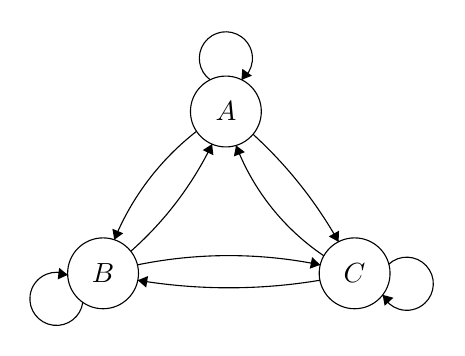
\begin{tikzpicture}[scale=0.15]
		\tikzstyle{every node}+=[inner sep=0pt]
		\draw [black] (23.7,-25.4) circle (3);
		\draw (23.7,-25.4) node {$A$};
		\draw [black] (13.3,-39.1) circle (3);
		\draw (13.3,-39.1) node {$B$};
		\draw [black] (34.6,-39.1) circle (3);
		\draw (34.6,-39.1) node {$C$};
		\draw [black] (14.249,-36.256) arc (157.70826:127.88572:22.39);
		\fill [black] (14.25,-36.26) -- (15.01,-35.71) -- (14.09,-35.33);
		\draw [black] (22.535,-28.163) arc (-25.83943:-48.56659:28.903);
		\fill [black] (22.53,-28.16) -- (21.74,-28.67) -- (22.64,-29.1);
		\draw [black] (16.213,-38.384) arc (101.57892:78.42108:38.549);
		\fill [black] (31.69,-38.38) -- (31,-37.73) -- (30.8,-38.71);
		\draw [black] (31.659,-39.688) arc (-80.52759:-99.47241:46.841);
		\fill [black] (16.24,-39.69) -- (16.95,-40.31) -- (17.11,-39.33);
		\draw [black] (25.997,-27.328) arc (47.64144:29.37151:36.624);
		\fill [black] (33.24,-36.43) -- (33.28,-35.49) -- (32.41,-35.98);
		\draw [black] (31.995,-37.618) arc (-123.95959:-159.02746:19.823);
		\fill [black] (24.56,-28.27) -- (24.38,-29.2) -- (25.31,-28.84);
		\draw [black] (22.377,-22.72) arc (234:-54:2.25);
		\fill [black] (25.02,-22.72) -- (25.9,-22.37) -- (25.09,-21.78);
		\draw [black] (37.487,-38.329) arc (132.69007:-155.30993:2.25);
		\fill [black] (36.97,-40.92) -- (37.14,-41.85) -- (37.88,-41.17);
		\draw [black] (11.585,-41.547) arc (-7.29476:-295.29476:2.25);
		\fill [black] (10.31,-39.23) -- (9.58,-38.63) -- (9.46,-39.62);
	\end{tikzpicture}
\end{center}


จากที่เรียนมาในห้อง เราทราบกันอยู่แล้วว่าความหมายของการนำเมทริกซ์การเปลี่ยนสถานะ 1 ขั้นมาคูณกัน จะได้ผลออกมาเป็นเมทริกซ์การเปลี่ยนสถานะข้าม 2 ขั้น (เช่นเปลี่ยนจากขั้นที่ 1 ไปขั้นที่ 3)
ดังนั้น ถ้าเราอยากหาผลคูณของเมทริกซ์การเปลี่ยนสถานะ สิ่งที่ต้องทำคือหาความน่าจะเป็นในการเดินข้าม 2 ขั้นทุกรูปแบบที่เป็นไปได้

\subsubsection*{การเปลี่ยนสถานะจาก A ในขั้นที่ 1 ไป A ในขั้นที่ 3}
วาดแผนภาพด้านล่าง โจทย์คือ \underline{\textbf{จงเขียนค่าความน่าจะเป็นของการย้ายสถานะของแต่ละเส้น (มี 6 เส้น)}}
\begin{center}
	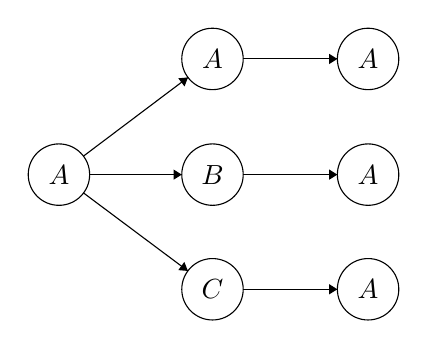
\begin{tikzpicture}[scale=0.13]
		\tikzstyle{every node}+=[inner sep=0pt]
		\draw [black] (11,-31.3) circle (3);
		\draw (11,-31.3) node {$A$};
		\draw [black] (26,-31.3) circle (3);
		\draw (26,-31.3) node {$B$};
		\draw [black] (26,-42.5) circle (3);
		\draw (26,-42.5) node {$C$};
		\draw [black] (26,-20) circle (3);
		\draw (26,-20) node {$A$};
		\draw [black] (41.2,-20) circle (3);
		\draw (41.2,-20) node {$A$};
		\draw [black] (41.2,-31.3) circle (3);
		\draw (41.2,-31.3) node {$A$};
		\draw [black] (41.2,-42.5) circle (3);
		\draw (41.2,-42.5) node {$A$};
		\draw [black] (13.4,-29.49) -- (23.6,-21.81);
		\fill [black] (23.6,-21.81) -- (22.66,-21.89) -- (23.27,-22.69);
		\draw [black] (14,-31.3) -- (23,-31.3);
		\fill [black] (23,-31.3) -- (22.2,-30.8) -- (22.2,-31.8);
		\draw [black] (13.4,-33.09) -- (23.6,-40.71);
		\fill [black] (23.6,-40.71) -- (23.25,-39.83) -- (22.66,-40.63);
		\draw [black] (29,-20) -- (38.2,-20);
		\fill [black] (38.2,-20) -- (37.4,-19.5) -- (37.4,-20.5);
		\draw [black] (29,-31.3) -- (38.2,-31.3);
		\fill [black] (38.2,-31.3) -- (37.4,-30.8) -- (37.4,-31.8);
		\draw [black] (29,-42.5) -- (38.2,-42.5);
		\fill [black] (38.2,-42.5) -- (37.4,-42) -- (37.4,-43);
	\end{tikzpicture}
\end{center}

ด้วยความรู้ในเรื่องความน่าจะเป็น เราจะได้ว่าความน่าจะเป็นรวมของการย้ายสถานะจาก A ข้ามไป A ใน 2 ขั้นถัดไปหาได้จากกฏการคูณและการบวกจากแผนภาพต้นไม้ดังกล่าว โดยที่
\begin{itemize}
	\item เส้นต่อกัน ให้นำค่าความน่าจะเป็นของเส้นมาคูณกัน
	\item หลังจากคิดผลคูณค่าความน่าจะเป็นของแต่ละกิ่งเรียบร้อยแล้ว ให้นำมาบวกกัน
\end{itemize}
เพราะฉะนั้น เราจะได้ว่าความน่าจะเป็นของการเปลี่ยนสถานะจาก A ข้ามไป A ใน 2 ขั้นถัดไปมีค่าเท่ากับ
$$
P(A\rightarrow_2A) = \left(\blank{1cm}\times\blank{1cm}\right) + \left(\blank{1cm}\times\blank{1cm}\right) + \left(\blank{1cm}\times\blank{1cm}\right) = 0.56
$$
ซึ่งมีผลลัพธ์เท่ากับสมาชิกในแถวที่ 1 หลักที่ 1 ที่แทนความน่าจะเป็นของการเปลี่ยนจาก A ไป A ในเมทริกซ์ผลลัพธ์
\subsubsection*{การเปลี่ยนสถานะจาก A ในขั้นที่ 1 ไป B ในขั้นที่ 3}
วาดแผนภาพด้านล่าง โจทย์คือ \underline{\textbf{จงเขียนค่าความน่าจะเป็นของการย้ายสถานะของแต่ละเส้น (มี 6 เส้น)}}
\begin{center}
	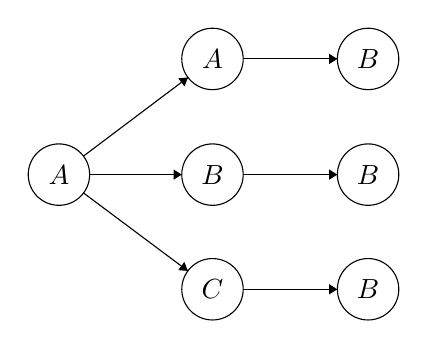
\begin{tikzpicture}[scale=0.13]
		\tikzstyle{every node}+=[inner sep=0pt]
		\draw [black] (11,-31.3) circle (3);
		\draw (11,-31.3) node {$A$};
		\draw [black] (26,-31.3) circle (3);
		\draw (26,-31.3) node {$B$};
		\draw [black] (26,-42.5) circle (3);
		\draw (26,-42.5) node {$C$};
		\draw [black] (26,-20) circle (3);
		\draw (26,-20) node {$A$};
		\draw [black] (41.2,-20) circle (3);
		\draw (41.2,-20) node {$B$};
		\draw [black] (41.2,-31.3) circle (3);
		\draw (41.2,-31.3) node {$B$};
		\draw [black] (41.2,-42.5) circle (3);
		\draw (41.2,-42.5) node {$B$};
		\draw [black] (13.4,-29.49) -- (23.6,-21.81);
		\fill [black] (23.6,-21.81) -- (22.66,-21.89) -- (23.27,-22.69);
		\draw [black] (14,-31.3) -- (23,-31.3);
		\fill [black] (23,-31.3) -- (22.2,-30.8) -- (22.2,-31.8);
		\draw [black] (13.4,-33.09) -- (23.6,-40.71);
		\fill [black] (23.6,-40.71) -- (23.25,-39.83) -- (22.66,-40.63);
		\draw [black] (29,-20) -- (38.2,-20);
		\fill [black] (38.2,-20) -- (37.4,-19.5) -- (37.4,-20.5);
		\draw [black] (29,-31.3) -- (38.2,-31.3);
		\fill [black] (38.2,-31.3) -- (37.4,-30.8) -- (37.4,-31.8);
		\draw [black] (29,-42.5) -- (38.2,-42.5);
		\fill [black] (38.2,-42.5) -- (37.4,-42) -- (37.4,-43);
	\end{tikzpicture}
\end{center}

เพราะฉะนั้น เราจะได้ว่าความน่าจะเป็นของการเปลี่ยนสถานะจาก A ข้ามไป B ใน 2 ขั้นถัดไปมีค่าเท่ากับ
$$
P(A\rightarrow_2B) = \left(\blank{1cm}\times\blank{1cm}\right) + \left(\blank{1cm}\times\blank{1cm}\right) + \left(\blank{1cm}\times\blank{1cm}\right) = \blank{1cm}
$$
\subsection*{โบนัสพิเศษ +1 คะแนน (แบบไม่หาร)}
จาก 2 ตัวอย่างที่ผ่านมา น่าจะพอสังเกตลักษณะการนำตัวเลขในเมทริกซ์มาคูณไขว้กันได้ จงอธิบายวิธีการคิดการคูณเมทริกซ์กับเมทริกซ์จากข้อสังเกตที่ได้ พร้อมทั้งแสดงวิธีคำนวณการคูณเพื่อหาสมาชิกอีก 7 ตัวที่เหลือ 
\newpage
\section*{Quiz 5}
สมมติว่าในการวิเคราะห์กลยุทธิ์การแข่งขันทางการตลาดแห่งหนึ่งแบบกลยุทธ์ผสม 2 กลยุทธ์ด้วยวิธีการวาดกราฟและได้กราฟดังรูป

\begin{tikzpicture}
	\begin{axis}[
		xmin=-0.1, xmax=1.1,
		ymin=-4.2, ymax=5.2,
		samples=200,
		domain=0:1,
		xlabel={$อัตราส่วนกลยุทธ์$}, ylabel={},
		xtick={0,1},
%		xticklabels={$x_1=0$,$x_1=1$},
		ytick={-4,-3,...,5},
		yticklabels={-4,-3,...,5},
		clip=false
		]
		
		% --- a family of light gray lines (candidates)
		\addplot[black!60] {-5*x+2};
		\addplot[black!60] {-2*x};
		\addplot[black!60] {4*x-1};
		\addplot[black!60] {9*x-4};
		
		
		% --- point at the "V" (where two branches meet), just for emphasis
		\addplot[only marks, mark=*, mark size=0.25pt] coordinates {(0.6667,-1.3333)};
		\node[anchor=north] at (axis cs:0.6667,-1.3333) {D};
		\addplot[only marks, mark=*, mark size=0.25pt] coordinates {(4/11,-8/11)};
		\node[anchor=north] at (axis cs:4/11,-8/11) {C};
		\addplot[only marks, mark=*, mark size=0.25pt] coordinates {(1/3,1/3)};
		\node[anchor=south] at (axis cs:1/3,1/3) {A};
		\addplot[only marks, mark=*, mark size=0.25pt] coordinates {(3/5,12/5 - 1)};
		\node[anchor=south] at (axis cs:3/5,12/5 - 1) {B};
		
		
		
		% --- thin verticals at x1=0 and x1=1 (as in the picture)
%		\addplot[black!50] coordinates {(0,-4.2) (0,5.2)};
		\addplot[black!50] coordinates {(1,-5.2) (1,6.2)};
		
		\addplot[black!50] coordinates {(0.975,5) (1.025,5)};
		\addplot[black!50] coordinates {(0.975,4) (1.025,4)};
		\addplot[black!50] coordinates {(0.975,3) (1.025,3)};
		\addplot[black!50] coordinates {(0.975,2) (1.025,2)};
		\addplot[black!50] coordinates {(0.975,1) (1.025,1)};
		\addplot[black!50] coordinates {(0.975,-1) (1.025,-1)};
		\addplot[black!50] coordinates {(0.975,-2) (1.025,-2)};
		\addplot[black!50] coordinates {(0.975,-3) (1.025,-3)};
		\addplot[black!50] coordinates {(0.975,-4) (1.025,-4)};
		
		% --- labels
		\node[anchor=west] at (axis cs:1,5) {$y=9p-4$};
		\node[anchor=west] at (axis cs:1,3) {$y=4p-1$};
		\node[anchor=west] at (axis cs:1,-2) {$y=-2p$};
		\node[anchor=west] at (axis cs:1,-3) {$y=-5p+2$};
		
		\node[anchor=west] at (axis cs:0,6) {$p=0$};
		\node[anchor=east] at (axis cs:1,6) {$p=1$};
		
	\end{axis}
\end{tikzpicture}

\begin{multicols}{2}
\noindent (1) จงแรเงาบริเวณการหา minimax พร้อมบอกจุดที่เป็น minimax ของการแข่งขันนี้ (A, B, C, หรือ D)
\begin{center}
	\begin{tikzpicture}
	\begin{axis}[
		xmin=-0.1, xmax=1.1,
		ymin=-4.2, ymax=5.2,
		samples=200,
		domain=0:1,
		xlabel={$อัตราส่วนกลยุทธ์$}, ylabel={},
		xtick={0,1},
		%		xticklabels={$x_1=0$,$x_1=1$},
		ytick={-4,-3,...,5},
		yticklabels={-4,-3,...,5},
		clip=false
		]
		
		% --- a family of light gray lines (candidates)
		\addplot[black!60] {-5*x+2};
		\addplot[black!60] {-2*x};
		\addplot[black!60] {4*x-1};
		\addplot[black!60] {9*x-4};
		
		
		% --- point at the "V" (where two branches meet), just for emphasis
		\addplot[only marks, mark=*, mark size=0.25pt] coordinates {(0.6667,-1.3333)};
		\node[anchor=north] at (axis cs:0.6667,-1.3333) {D};
		\addplot[only marks, mark=*, mark size=0.25pt] coordinates {(4/11,-8/11)};
		\node[anchor=north] at (axis cs:4/11,-8/11) {C};
		\addplot[only marks, mark=*, mark size=0.25pt] coordinates {(1/3,1/3)};
		\node[anchor=south] at (axis cs:1/3,1/3) {A};
		\addplot[only marks, mark=*, mark size=0.25pt] coordinates {(3/5,12/5 - 1)};
		\node[anchor=south] at (axis cs:3/5,12/5 - 1) {B};
		
		
		
		% --- thin verticals at x1=0 and x1=1 (as in the picture)
		%		\addplot[black!50] coordinates {(0,-4.2) (0,5.2)};
		\addplot[black!50] coordinates {(1,-5.2) (1,6.2)};
		
		\addplot[black!50] coordinates {(0.975,5) (1.025,5)};
		\addplot[black!50] coordinates {(0.975,4) (1.025,4)};
		\addplot[black!50] coordinates {(0.975,3) (1.025,3)};
		\addplot[black!50] coordinates {(0.975,2) (1.025,2)};
		\addplot[black!50] coordinates {(0.975,1) (1.025,1)};
		\addplot[black!50] coordinates {(0.975,-1) (1.025,-1)};
		\addplot[black!50] coordinates {(0.975,-2) (1.025,-2)};
		\addplot[black!50] coordinates {(0.975,-3) (1.025,-3)};
		\addplot[black!50] coordinates {(0.975,-4) (1.025,-4)};
		
		
	\end{axis}
\end{tikzpicture}
\end{center}

\noindent (2) จงแรเงาบริเวณการหา maximin พร้อมบอกจุดที่เป็น maximin ของการแข่งขันนี้ (A, B, C, หรือ D)
\begin{center}
	\begin{tikzpicture}
	\begin{axis}[
		xmin=-0.1, xmax=1.1,
		ymin=-4.2, ymax=5.2,
		samples=200,
		domain=0:1,
		xlabel={$อัตราส่วนกลยุทธ์$}, ylabel={},
		xtick={0,1},
		%		xticklabels={$x_1=0$,$x_1=1$},
		ytick={-4,-3,...,5},
		yticklabels={-4,-3,...,5},
		clip=false
		]
		
		% --- a family of light gray lines (candidates)
		\addplot[black!60] {-5*x+2};
		\addplot[black!60] {-2*x};
		\addplot[black!60] {4*x-1};
		\addplot[black!60] {9*x-4};
		
		
		% --- point at the "V" (where two branches meet), just for emphasis
		\addplot[only marks, mark=*, mark size=0.25pt] coordinates {(0.6667,-1.3333)};
		\node[anchor=north] at (axis cs:0.6667,-1.3333) {D};
		\addplot[only marks, mark=*, mark size=0.25pt] coordinates {(4/11,-8/11)};
		\node[anchor=north] at (axis cs:4/11,-8/11) {C};
		\addplot[only marks, mark=*, mark size=0.25pt] coordinates {(1/3,1/3)};
		\node[anchor=south] at (axis cs:1/3,1/3) {A};
		\addplot[only marks, mark=*, mark size=0.25pt] coordinates {(3/5,12/5 - 1)};
		\node[anchor=south] at (axis cs:3/5,12/5 - 1) {B};
		
		
		
		% --- thin verticals at x1=0 and x1=1 (as in the picture)
		%		\addplot[black!50] coordinates {(0,-4.2) (0,5.2)};
		\addplot[black!50] coordinates {(1,-5.2) (1,6.2)};
		
		\addplot[black!50] coordinates {(0.975,5) (1.025,5)};
		\addplot[black!50] coordinates {(0.975,4) (1.025,4)};
		\addplot[black!50] coordinates {(0.975,3) (1.025,3)};
		\addplot[black!50] coordinates {(0.975,2) (1.025,2)};
		\addplot[black!50] coordinates {(0.975,1) (1.025,1)};
		\addplot[black!50] coordinates {(0.975,-1) (1.025,-1)};
		\addplot[black!50] coordinates {(0.975,-2) (1.025,-2)};
		\addplot[black!50] coordinates {(0.975,-3) (1.025,-3)};
		\addplot[black!50] coordinates {(0.975,-4) (1.025,-4)};
		
	\end{axis}
\end{tikzpicture}
\end{center}
\end{multicols}

\subsection*{โบนัสพิเศษ +1 คะแนน (แบบไม่หาร)}
จงแก้สมการหาค่าพิกัดของจุด maximin ที่ระบุในข้อ (2) (หาค่า p ได้จะได้ 0.5 คะแนน) พร้อมทั้งระบุค่าของเกม (หาค่าของเกมได้จะได้ 0.5 คะแนน)
\newpage